\section{A quick overview}
Both stacks and queues are quite basic data structures,
and their functionality can be implemented to run very fast. 
They often serve key (if simple) roles in algorithms and inside
computer systems.
And it is surprising how much actually interesting
behavior can be obtained from just such simple structures.

A \todef{queue} is the natural analogue of a line at a store%
\footnote{In fact, in British English, the word ``queue'' means
  ``line;'' people there ``queue up'' in grocery stores instead of
  ``lining up.''}: 
elements arrive one by one, get in the queue, and are removed from the
queue in the order in which they arrived.
This makes the order of a queue FIFO (first in, first out).
Specifically, the functionality of a queue is the following:

\begin{itemize}
\item add an element.
\item look at the oldest element.
\item remove the oldest element.
\end{itemize}

We can visualize a queue like a conveyor belt on which we place the
elements.
One of the main uses of queues (outside of something like simulating a
store) is to manage access to shared resources (such as a printer or
processor).
In fact, printers traditionally have a queue implemented on a server:
when users try to print documents, those are added to the queue,
and when the printer finishes a previous job, the next job is chosen
by the order in which the jobs were received. 

\medskip

A \todef{stack} is the natural analogue of piling papers, boxes, or
other important things on top of each other.
At any time, we can only access the most recently added item,
which sits on top.
To get at the others, we first need to take care of and remove the
more recent ones. 
This makes a stack LIFO (last in, first out).
The functionality of a stack is the following:

\begin{itemize}
\item add an element.
\item look at the most recently added element.
\item remove the most recently added element.
\end{itemize}

A stack is often drawn in analogy with a physical stack of boxes/papers.
Most of a program's variables (everything we do not put on the heap) are
kept on the program stack.
When one function in a program calls another (or itself), all its
variables (and state) are saved on the stack, and then the next function starts.
We always have to finish the execution of the current function
(and remove its variables) before we can access the variables of the
other functions (those that called this function).
Thus, by explicitly implementing a stack, we can get rid of recursion
(which is what really happens in compiling a program).

Stacks are particularly useful when parsing programs or other types of
recursively defined expressions.
In fact, we will see an easy example momentarily.
Another real-world example is the hiring/firing practices at LAUSD:
when teachers need to be laid off due to budget shortages,
the current rule is that the most recently hired teachers are laid off
first.
One may argue whether this is a reasonable rule,
but it does implement a stack.

\section{Stacks}
As we said before, stacks are used internally by the compiler for
implementing recursion; generally, they are useful for computations
that proceed ``inside out,'' as we will see below.

Assume that our stack stores elements of some type \code{T}.
The functionality that a stack offers us more formally is the following: 
\begin{itemize}
% DK: Used to have "const T & data". const is only introduced later.
\item Adding an element: \code{void push (T \& data)}
\item Look at the top (most recently added) element:
\code{T top ()} (also sometimes, for instance in the textbook, called
\code{T peek ()}).
\item Remove the top (most recently-added) element:
\code{void pop()}.
\end{itemize}
Notice that the only element that we can look at or remove is the one
on top of the stack.
Also, in practice, to make the stack easier to use,
you would probably add a function \code{bool isEmpty()} which
returns whether there are any elements on the stack.
But the three functions given above are really what makes a stack a stack.

As with other data structures we have seen so far,
we would like to define formally what is and is not a stack.
As before, a recursive definition is perhaps clearest and simplest:
A stack is either
\begin{enumerate}
\item the empty stack, or
\item of the form \code{S.push(data)}, where \code{S} is a stack, and
  \code{data} is a data item.
\end{enumerate}

This tells us what is and is not a stack, but it does not tell us the
semantics of the stack functions, i.e., what exactly they do. 
The nice thing about stacks is that they are simple enough that we
can completely specify the meaning of their functions using formulas.
Some people would call these formulas the \todef{stack axioms}:

\begin{enumerate}
\item For all stacks S: S.push(data).top() = data.
\item For all stacks S: S.push(data).pop() = S.
\end{enumerate}

This says that if you read the top element after pushing something on
a stack, you get that element back.
And if you remove the top element after pushing something on the stack,
you get the original stack back.
The definition does not say what happens when you call \code{pop} or
\code{top} on an empty stack.
(In other words, we do not define \code{pop} or \code{top} for the
base case of our recursive stack definition.)
This is intentional: there is no real ``correct'' meaning that we
could assign those operations.
When you implement a stack, of course you will have to choose what happens,
and you should document your choice. 
But behavior for cases that really should not happen is not really
something that needs to go in a high-level definition of an abstract
data type, and someone who plans to use a stack to solve a problem to
solve some bigger algorithmic problems should not rely on specific
behavior for faulty inputs.

A second thing to reiterate is that it is really quite amazing that
the stack functionality can be completely specified with two lines of
math, and two simple lines at that.
When we get to queues later, this will not be possible.
At an intuitive level, for a stack, adding and removing come in pairs
that are right next to each other, while for queues, there can be
arbitrarily many elements between adding an element and seeing it again.
This means that to specify the semantics of queue operations,
one has to use more advanced mathematical specifications.

At an even more philosophical level, this difference is why many
mathematically inclined people prefer functional programming.
Recursion by nature resembles stacks: the behavior of a function can
be summarized, and then substituted where it occurs.
Analyzing \code{for} loops, on the other hand, requires something
called fixed point operators, which is much less intuitive.
As a result, carefully thought through recursive solutions are often
much more robust.

\subsection{Example}
As an example of something that is really easy to do with stacks, and
would not at all be obvious without stacks or recursion, let us look at
the following task:
You are given a string of characters: 
lowercase letters and opening and closing parentheses, brackets, and
braces ``( [ \{ \} ] )''. 
The goal is to test if all of the parentheses/square brackets/braces match.
To illustrate the task, here are some examples:
\begin{enumerate}
\item ``([ab\{c\}]de())'' is correct: all opening/closing
  braces match.
\item ``([ab]]'' is incorrect: the closing square bracket does not
  match the opening parenthesis.
\item ``ab\}'' is incorrect: there is no opening brace matching the
  closing one.
\end{enumerate}
		
We now outline an algorithm (using a stack) to recognize whether the
string has matching parentheses and brackets and braces.

\begin{enumerate}
\item The stack starts out empty.
\item The string is scanned character by character, left to right.
\begin{itemize}
\item Each time an opening brace/bracket/parenthesis is encountered,
  push it onto the stack.
\item When a letter is encountered, ignore it.
\item When there is a closing brace/bracket/parenthesis, 
check if it matches what is on top of the stack. 
\begin{itemize}
\item If it does, then pop the matching brace/bracket/parenthesis off the
stack. 
\item If it does not, then output that this is bad input (mismatch).
\item If the stack was empty, then output a bad input (missing opening
  parenthesis).
\end{itemize}
\end{itemize}
\item If the stack is not empty at the end, there was an unmatched
  opening parenthesis/bracket/brace, so output an error.
\end{enumerate}

In a sense, we can regard the above algorithm as a very rudimentary
parser. It is easy to imagine putting numbers to add or multiply in
there, or putting C++ code inside the braces.
Indeed, most implementations of parsers for languages (programming
languages, logic formulas, arithmetic expressions, $\ldots$) use
stacks either explicitly or at least implicitly (through recursion).

When you use the preceding techniques to write a parser for formulas
(e.g., a simple calculator, or a parser for a programming language, or
for Boolean formulas), you would go one step further: whenever you
encounter a closing parenthesis, you know that you reached the end of
an expression that you are now ready to evaluate. Typically, you would
now pop stuff off the stack until you have the entire internal
expression, and instead push its value back on the stack. That way,
you evaluate the formula inside out.

Looking ahead a little bit to proving correctness of algorithms
formally, we would like to argue that the algorithm does the right
thing. Of course, it is our intuition that it does --- otherwise, we
would not have come up with this algorithm. But sometimes, we make
mistakes, not just in our implementation, but also in our logic.

There are techniques for mathematically proving that a
program/algorithm is correct.
These are based on phrasing axioms about what exactly certain
programming constructs do, such as our axioms about the stack
functions above.
Whenever a program contains recursion or loops, such proofs are
invariably based on using induction.
For loops, a key element of a correctness proof by induction is what is
called a \todef{loop invariant}: a property that will be true after
each iteration of the loop, such that it is trivial that is true at the
beginning (base case), and if we can prove that it holds at the end,
our program has done the correct thing.
Then, proving that the invariant holds from one loop to the next is
exactly the induction step of a proof by induction. 

While we will not do a full correctness proof by induction for this
algorithm, for the curious student, the following should be pointed out:
the algorithm runs a loop over all characters of the input string.
The important part of the loop invariant is that at any time, the top
of the stack is the most recent unmatched opening parenthesis/bracket/brace.
If one were to really attempt the proof,
this is not enough to make the induction step work.
The actual hypothesis needed is the following: at any stage of the
processing, the stack contains all currently unmatched parentheses, in
right-to-left order (top-to-bottom in the stack).

\subsection{Implementation of a general-purpose stack}

A stack can be naturally (and quite easily) implemented using either a
linked list or an array (so long as we dynamically resize it, the way we
suggested for implementing a \code{List}).

For an implementation based on linked lists, we could insert and
delete either at the head or tail. Both are roughly equally easy to
implement, though inserting and deleting at the head may be even
easier, because even a singly-linked list will do:
\begin{itemize}
\item To push an item, create a new element, link it to the old head,
  and make it the new head.
\item To read the top, return the head's data item.
\item To pop off the stack, remove the head from the list, and set its
  next element as the new head.
\end{itemize}
Notice that for none of these operations do we ever need to access any
element's previous element. 
We could also perform similar operations on the tail of a linked
list, but in order to pop the last element, we need to know its
predecessor, which will be the new tail; so we would need a doubly
linked list, or to scan through the entire list to find the new tail.
The latter would of course be inefficient.

An implementation using arrays is not much more difficult:
we have an array \code{a} and store the size of the stack in some
variable, say, called \code{size}.
\begin{itemize}
\item To push an item, we write it into \code{a[size]} and increment
  \code{size}. If we now exceed the allocated array size, we expand the
  array by allocating a new larger array and copying the data over,
  much like we did for the \code{List} datatype.
\item To read the top, we simply return \code{a[size-1]}.
\item To pop an element off the stack, we decrement the size.
\end{itemize}

For both implementations, the running time of the \code{top} and
\code{pop} operations is clearly $O(1)$, as we only return a directly
accessible element, and update only a constant number of pointers or
integer variables.
For \code{push}, the linked list implementation is also clearly $O(1)$.
For the array implementation, it is $O(1)$ except when the
array size has to increase (in which case it is $\Theta(n)$).
However, if we double the array size every time the array is too small
(rather than, say, incrementing it only by 1), then for every
operation that takes $\Omega(n)$, the next $n$ operations will
require no doubling and thus take $O(1)$,
as we discussed in Chapter~\ref{arraylists}.
In total, those $n+1$ operations thus take $O(n)$,
which means that on average, they take $O(1)$. 
This is another example of ``amortized analysis.''

\section{Queues}

Recall that queues provide ``First In First Out'' (FIFO) access to data. 
When elements are added into a queue, they can be read/removed only in
exactly the order in which they were added.
The functionality of queues (storing elements of some type \code{T})
is the following:

\begin{itemize}
\item Adding an element: 
% DK: Used to say "const T & data". const is only introduced later.
\code{void enqueue (T \& data)}.
\item Look at the oldest element in the queue: 
\code{T peekfront ()}.
\item Remove the oldest element from the queue:
\code{void dequeue ()}.
\end{itemize}

As with stacks, you would likely want to add a function \code{bool isEmpty()}
in practice.
Notice again the contrast to stacks: with a stack,
you can only access (read/remove) the most recently added element,
while a queue only allows you to access the oldest element.

Much like with stacks, we can define formally what is and is not a queue.
A queue is either:
\begin{enumerate}
\item the empty queue, or
\item of the form \code{Q.enqueue(data)}, where \code{Q} is a queue,
  and \code{data} is a data item.
\end{enumerate}

As we discussed above, the precise semantics of the operations on a
queue are much harder to specify, and far beyond what we can do in
this class.
%(And unfortunately, at USC, we do not have a class on
%semantics of programming languages.)

\subsection{Implementation of a queue}
Just like with a stack,
a queue can be implemented using a linked list or an array.

For an implementation using linked lists, we have two choices: 
(1) insert at the head and read/remove at the tail, or
(2) insert at the tail and read/remove at the head.
There is a slight advantage to the second version,
because a singly linked list suffices:
when we delete, we only need to set
\code{head=head->next} (and deallocate the old \code{head}).
In order to delete at the tail, we would need to know the tail's
predecessor,
which would require a doubly linked list or a linear-time search.

For an implementation using arrays, compared to stacks, we now need
two integer indices: one (say, \code{newest}) for the position of the
newest element in the array, and one (say, \code{oldest}) for the
position of the oldest element. 
When enqueueing a new element,
we can write it into \code{a[newest]} and increment \code{newest}.
To implement \code{peekfront}, we can return \code{a[oldest]};
and to dequeue the oldest element,
we can just increment \code{oldest} by one.
As before, when enqueueing a new element and exceeding the current
array size, we need to expand the array.

One downside of this implementation is that it may be quite wasteful
of space.
In particular if the queue is used for a long time, after a while,
both \code{newest} and \code{oldest} may be large,
which means that most of the array is unused.
Instead, we could have the array ``wrap around,''
by doing calculations of the index \code{newest} modulo the array's size.
This makes better use of space, but we now have to be careful not to
overwrite the older elements with newer elements.
None of this is a huge obstacle, but one has to be a bit more careful
in the implementation, which perhaps makes an implementation based on linked
lists slightly more attractive.

The running time analysis is pretty much identical to the one for a
stack.
All operations are $O(1)$ because they just involve updates of a small
number of variables.
As before, the only exception is the possible expansion of the array,
which may take $\Theta(n)$,
and which can again be amortized if the array size doubles
(or gets \emph{multiplied} with some number $b > 1$, rather than
having something \emph{added} to it) whenever the array is too small. 

\section{Why use restrictive data structures?}
As we saw, a stack only allows access to the most recently
added element, while a queue only allows access to the oldest element
in the data structure.
Could we have a data structure that allows access to either, as we need it?

Indeed, we can.
There is a data structure called \code{Deque},
which does exactly that:
it allows adding and accessing (reading/removing) elements at both ends.
If you understood how to implement a stack and a queue,
implementing a \code{Deque} will be easy for you.
So why would we not use a \code{Deque} everywhere instead of stacks or
queues?

Or, perhaps more strongly: why don't we just use the C++ \code{vector}
class for all data structures?
It combines the functionality of a stack, queue, and \code{List} in
the sense in which we defined it in previous lectures.
So it is much more powerful.

One answer to this question is pedagogical: in this class, we want to
learn how these data structures work internally, and using a powerful
tool without understanding it does not contribute to learning.

A second answer is relevant when we have to implement the data
structures ourselves:
if a data structure provides more functions,
then it is more work to implement,
and offers more places to make implementation mistakes.
So if we implement data structures ourselves,
there is something to be said for keeping our data structures simple.
But of course, that argument does not apply when we use data
structures provided as part of a programming language.

A third, and often appropriate, answer is that in order to implement
more functions, the implementation of other functions may be less
efficient. For instance, in order to allow access to each element in
constant time, \code{vector} is implemented internally as an array.
That may slow down the implementation of some other functions,
which could be implemented faster if we did not also need access by
index.

The fourth, and real, answer lies in our goal of writing code that we
and our collaborators can understand easily in the future. 
If you write code in which you explicitly use a variable of type
\code{Stack}, you make it clear that all your code needs is the
\code{Stack} functionality, which will help others
(and yourself, if you return to your code weeks or months later)
parse the logic of your code.
If instead, you had used \code{Deque} or \code{Vector} types,
others may wonder whether somewhere buried in line 1729 of your code,
you actually access specific elements, or need to access both the head
and tail of your \code{Deque}. That makes it harder to understand the
logic. So in general, it is a good idea to think through your code's
logic ahead of time, and only declare those data structures that you
really need.

\begin{figure}[htb]
\centering
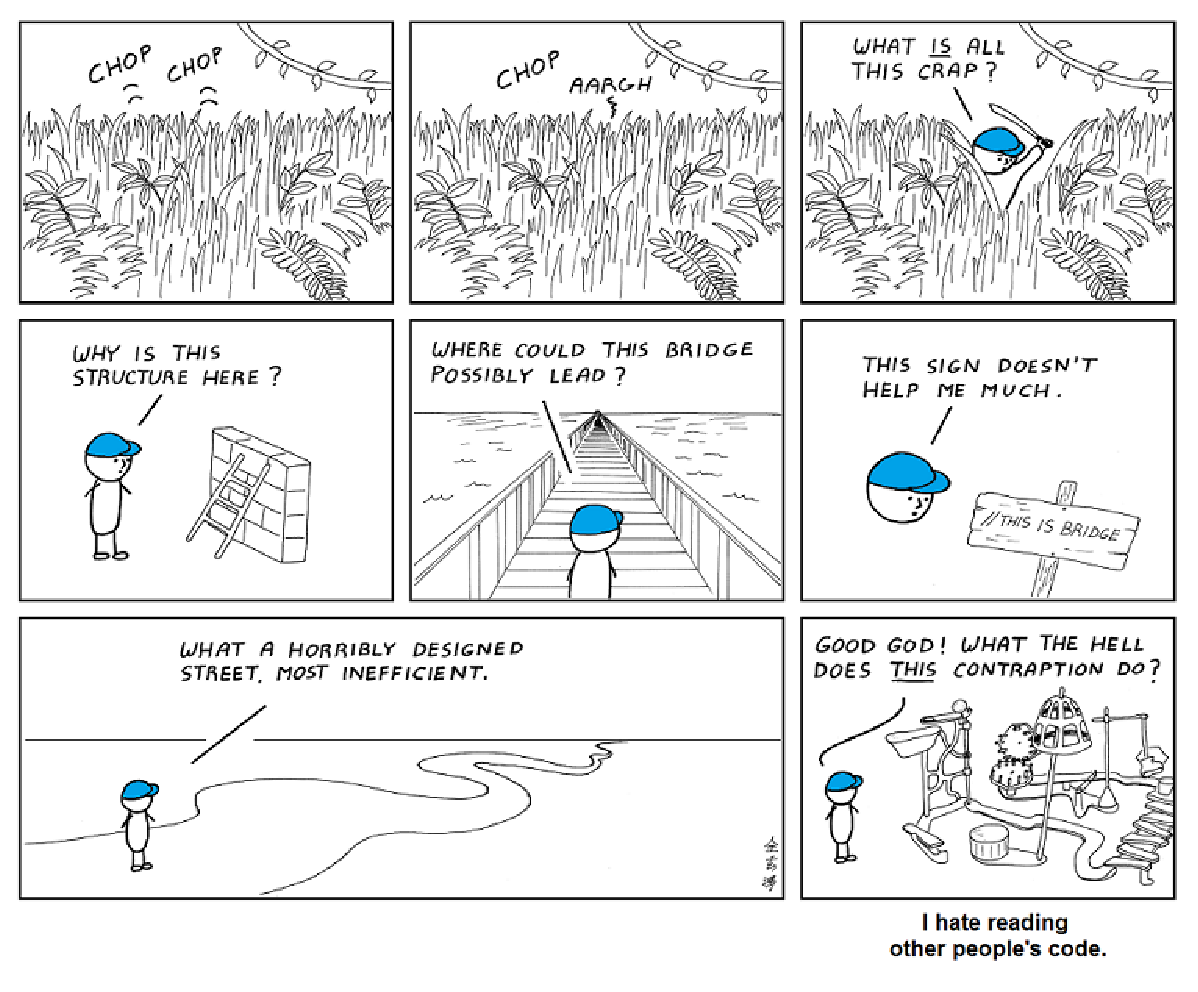
\includegraphics[scale=0.4]{comics/abstruse_goose_opc.eps}
\caption{Abstruse Goose \# ???: OPC}
\end{figure}

You could of course try to make this clear with
our variable names, say, by writing something like
\code{vector<int> stack}.
If you do this, it might convey your intention.
But of course, another interpretation would be that you had initially
written \code{Stack<int> stack}, and then later realized that you actually
needed extra functionality. But because you did not want to rename the
variable everywhere, you just changed its type to \code{vector<int>},
so even though the variable is called \code{stack}, it is not actually
used as one.

The upshot is that you should ideally declare your variables to be
of the type that you actually need, not giving yourself extra
functionality you do not intend to use. 
In particular, you may not find too many immediate uses for a
\code{Deque},
since most of the time, you will want either a \code{Stack} or \code{Queue}.
